\documentclass[tikz,border=3mm]{standalone}

\usepackage{optikz}
\usepackage{tikz}
\usetikzlibrary{arrows.meta,calc,positioning}

\tikzset{
  beam/.style={-Latex, line width=0.9pt},
  lab/.style={font=\sffamily\small},
  smallbox/.style={
    draw,
    rounded corners=1pt,
    minimum height=7mm,
    minimum width=14mm,
    align=center,
    font=\sffamily\small
  }
}

\begin{document}
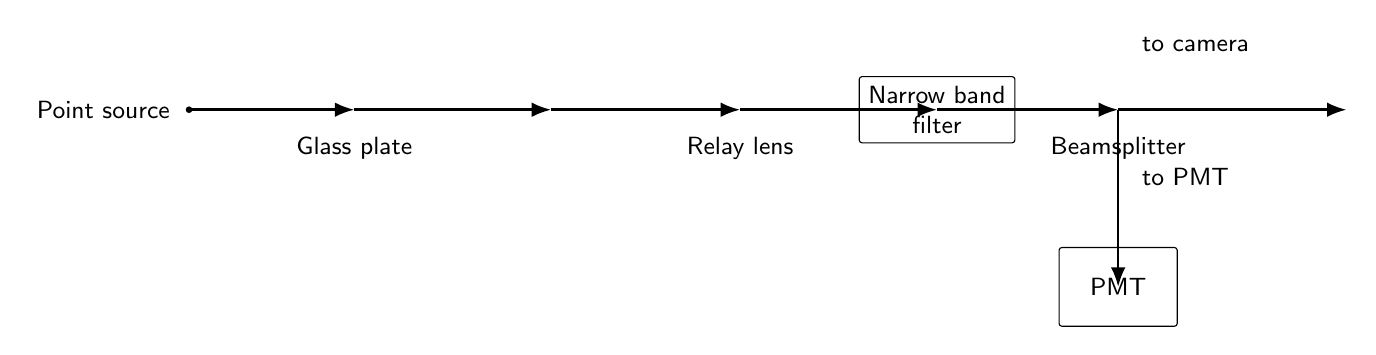
\begin{tikzpicture}[x=1cm,y=1cm]

% --- coordinates ---
\coordinate (src)    at (0,0);
\coordinate (plate)  at (2.1,0);
\coordinate (obj)    at (4.6,0);
\coordinate (relay)  at (7.0,0);
\coordinate (filter) at (9.5,0);
\coordinate (bs)     at (11.8,0);
\coordinate (pmt)    at (11.8,-2.25);
\coordinate (cam)    at (14.7,0);

% --- beam path ---
\draw[beam] (src) -- (plate);
\draw[beam] (plate) -- (obj);
\draw[beam] (obj) -- (relay);
\draw[beam] (relay) -- (filter);
\draw[beam] (filter) -- (bs);
\draw[beam] (bs) -- (cam);
\draw[beam] (bs) -- (pmt);

% --- source ---
\fill (src) circle (1.2pt);
\node[lab, anchor=east] at ($(src)+(-0.12,0)$) {Point source};

% --- glass plate ---
\splitter[width=0.28, thickness=0.9] at (plate);
\node[lab, below=2.2mm] at (plate) {Glass plate};

% --- HNA objective ---
\objective[name={HNA\\objective}] at (obj);

% --- relay lens ---
\convexlens[width=0.85] at (relay);
\node[lab, below=2.2mm] at (relay) {Relay lens};

% --- narrow band filter ---
\node[smallbox, minimum width=19mm, minimum height=8mm] at (filter) {Narrow band\\filter};

% --- beamsplitter ---
\splitter[width=0.34, thickness=0.95] at (bs);
\node[lab, below=2.2mm] at (bs) {Beamsplitter};

% --- detectors ---
\camera[name={CMOS\\camera}] at (cam);
\node[smallbox, minimum width=15mm, minimum height=10mm] at (pmt) {PMT};

% --- branch labels ---
\node[lab, anchor=south west] at ($(bs)+(0.18,0.62)$) {to camera};
\node[lab, anchor=north west] at ($(bs)+(0.18,-0.62)$) {to PMT};

\end{tikzpicture}
\end{document}
